\section{Сортировка Шелла}

\subsection{Принцип работы}

При сортировке Шелла сначала сравниваются и сортируются между собой значения, стоящие один от другого на некотором расстоянии $d$.
После этого процедура повторяется для некоторых меньших значений $d$, а завершается сортировка Шелла упорядочиванием элементов при $d = 1$ (то есть обычной сортировкой вставками).
Эффективность сортировки Шелла в определённых случаях обеспечивается тем, что элементы «быстрее» встают на свои места (в простых методах сортировки, например, пузырьковой, каждая перестановка двух элементов уменьшает количество инверсий в списке максимум на 1, а при сортировке Шелла это число может быть больше).

Для определённости будет рассматриваться классический вариант, когда изначально $d = \frac{n}{2}$ и уменьшается по закону $d_{i+1} = \frac{d_{i}}{2}$, пока не достигнет $1$. 
Здесь $n$ обозначает длинну сортируемого массива.

Тогда в худшем случае сортировка займет $O(n^2)$.

Блок схема сортировки Шелла:\\
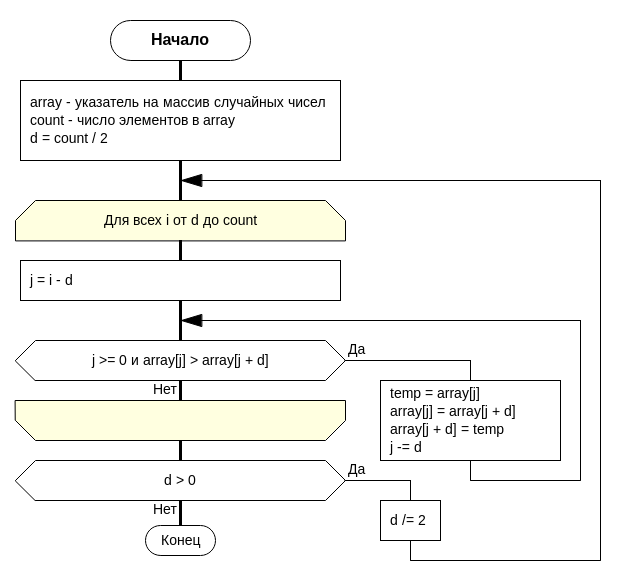
\includegraphics[scale=0.6]{res/original.png}

\subsection{Параллелизация}

Как и в предыдущих лабораторных, в первую очередь параллелизируется цикл.

Задаем число потоков и общие переменные через \textit{omp parallel}.
Однозначно общими должны быть массив и его длинна.

Так как внутренний цикл по i по сути затрагивает только $d$-e элементы отностительно $i$-го, то его можно параллелизировать:

\begin{lstlisting}[language=C, basicstyle=\scriptsize]
 #pragma omp parallel num_threads(THREADS) shared(array, count) default(none)
    for (int d = count / 2; d > 0; d /= 2) {
        const int cd = d;
        #pragma omp for
        for (int i = cd; i < count; ++i) {
            for (int j = i - cd; j >= 0 && array[j] > array[j + cd]; j -= cd) {
                int temp = array[j];
                array[j] = array[j + cd];
                array[j + cd] = temp;
            }
        }
    }
\end{lstlisting}

Здесь так же видно, что $d$ вынесена в константу $cd$.
Это сделано для того, что бы \textit{OpenMP} не принял меры предосторожности в цикле по $i$.
Он может это сделать так как $d$ меняется во внешнем цикле, но он не знает меняется ли во внутреннем.